

\begin{figure*}[htbp]
    \centering
    \begin{tabular}{m{68mm} m{70mm} m{10mm}}
        % First row: Image 1, 2, and vertically spanning Image 5
        \begin{minipage}[b]{70mm}
            \centering
            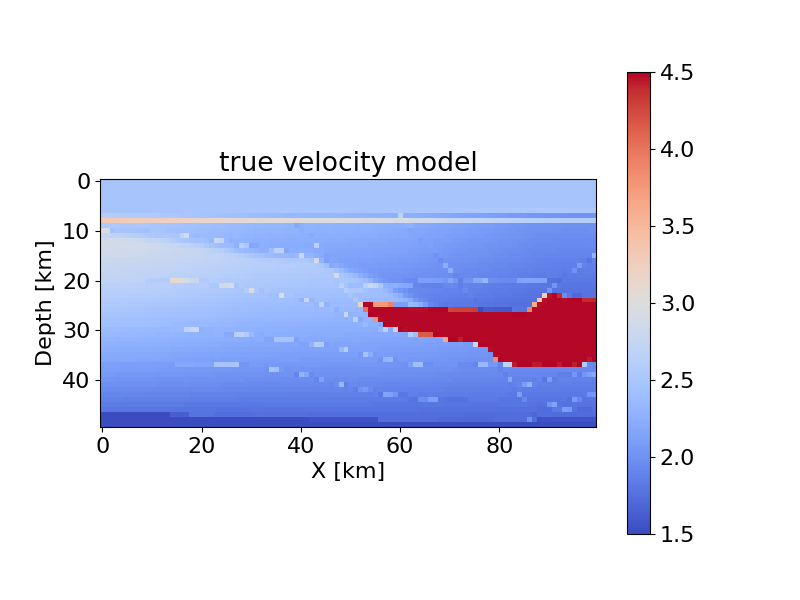
\includegraphics[width=70mm]{public/true}
            \caption*{\raisebox{5mm}{Background truth}}
        \end{minipage} &
        \begin{minipage}[b]{70mm}
            \centering
            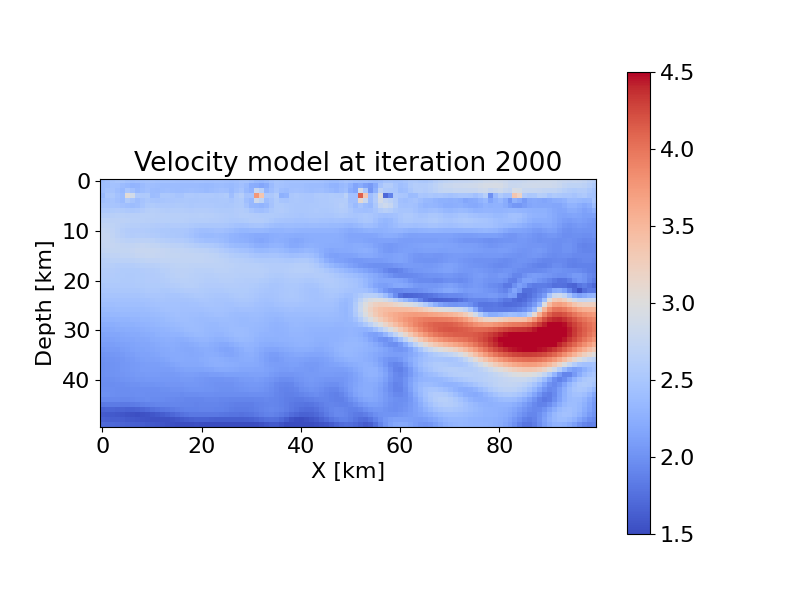
\includegraphics[width=70mm]{public/gradient}
            \caption*{\raisebox{5mm}{Reconstructed with standard FWI}}
        \end{minipage} &
        \multirow[t]{2}{*}{\raisebox{-50mm}{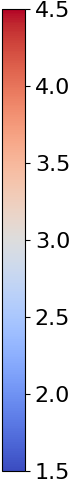
\includegraphics[height=68mm]{public/color-bar}}} \\
        % Second row: Image 3 and 4
        \begin{minipage}[b]{70mm}
            \centering
            
\includegraphics[width=70mm]{public/initial}
            \caption*{Initial model}
        \end{minipage} &
        \begin{minipage}[b]{70mm}
            \centering
            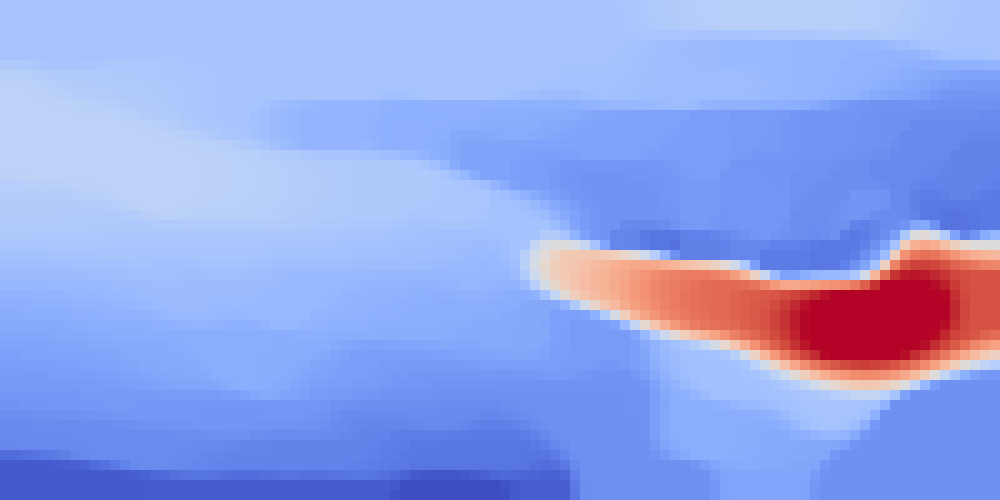
\includegraphics[width=70mm]{public/pds}
            \caption*{Reconstructed with the constrained FWI}
        \end{minipage} &
    \end{tabular}
    \caption{Velocity models and their corresponding reconstructions.}
    \label{fig:velocity-models}
\end{figure*}


\subsection{Experimental Setup}\label{subsec:experimental-setup}

To demonstrate the effectiveness of the TV and box constrained FWI, we conducted experiments where we compared with the standard FWI with gradient method~\eqref{eq:FWIWithGradient}, using the SEG/EAGE Salt and Overthrust Models.
The velocity model consists of 101 $\times$ 51 grid points.
The ground truth velocity model is generated by zooming and cropping Fig.\ref{fig:salt-model}, and the initial velocity model is generated by smoothing the ground truth velocity model with a Gaussian function with a standard deviation of 80.
The number of receivers and source shots are 101 and 20, respectively, and are placed on the surface at equal intervals.
The source waveform is a Ricker wavelet with a peek wavelet frequency of 10 Hz.
The gradient of $E$ is computed numerically using the Devito framework\cite{devito}.
In the standard FWI, the step size $\gamma$ is set to $1.0 \times 10^{-4}$.
In the TV and box constrained FWI, the step size $\gamma_1$ and $\gamma_2$ are set to $1.0 \times 10^{-4}$ and $1.0 \times 10^2$, respectively, the upper bound of the $l_{1,2}$ norm $\alpha$ is set to 340, and the lower and upper bounds of the velocity model $a$, $b$ are set to 1.5[km/s] and 4.5[km/s], respectively.
The number of iterations is set to 5000.


\subsection{Results and Discussion}\label{subsec:results-and-discussion}

Fig.\ref{fig:velocity-models} shows the ground truth, the initial model, and the reconstructed velocity models using the standard FWI and the TV and box constrained FWI.
It can be observed that the TV and box constrained FWI successfully eliminates wave-like artifacts and noise that appear at the source positions, resulting in a more accurate velocity model reconstruction.

In Fig.\ref{fig:ssim}, we plot the Structural Similarity Index Measure (SSIM) against the number of iterations for both methods.
The proposed method consistently achieves higher SSIM values than the standard FWI at every iteration, indicating improved reconstruction quality.

Furthermore, since the computational bottleneck lies in the gradient computation of $E$, the introduction of the constraints does not significantly affect the overall computational cost.
This demonstrates that the proposed method enhances reconstruction accuracy without incurring additional computational costs.

However, it should be noted that parameters such as $\alpha$, $a$, and $b$ were determined by referencing the ground truth data.
While this experiment shows that good results can be achieved by appropriately setting these parameters, they need to be determined independently of this framework in practical applications.


\begin{figure}[htbp]
\vspace{-\baselineskip}
\begin{center}
    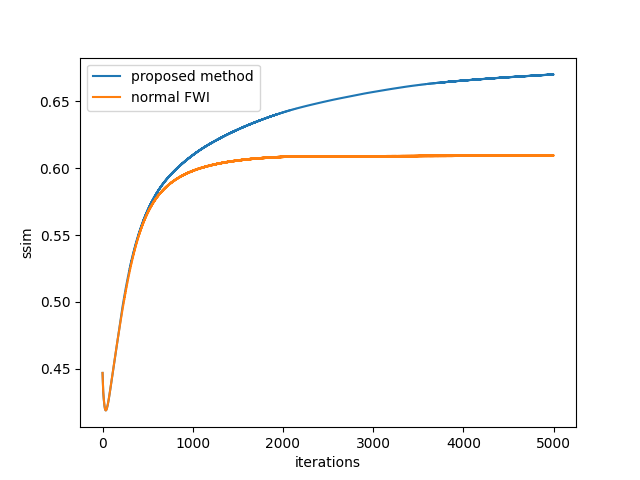
\includegraphics[width=80mm]{public/ssim}
    \caption{SSIM against the number of iterations.}
    \label{fig:ssim}
\end{center}
\vspace{-\baselineskip}
\end{figure}
